\documentclass[12pt]{article}
\usepackage{graphicx}

% \addtolength{\oddsidemargin}{-.875in}
% \addtolength{\evensidemargin}{-.875in}
% \addtolength{\textwidth}{1.75in}
\addtolength{\oddsidemargin}{-.4375in}
\addtolength{\evensidemargin}{-.4375in}
\addtolength{\textwidth}{0.875in}

% \addtolength{\topmargin}{-.875in}
% \addtolength{\textheight}{1.75in}
\addtolength{\topmargin}{-.4375in}
\addtolength{\textheight}{0.875in}

\def\yis{$\Upsilon(1S)$}
\def\yiis{$\Upsilon(2S)$}
\def\yiiis{$\Upsilon(3S)$}
\def\yivs{$\Upsilon(4S)$}
\def\yvs{$\Upsilon(10860)$}
\def\yvis{$\Upsilon(11020)$}
\def\gamee{$\Gamma_{ee}$}
\def\gamtot{$\Gamma$}
\def\gamofw{$\Gamma(w)$}
\def\gamtotot{$\Gamma_{\Upsilon\ \to \mbox{ anything}}$}
\def\bree{$\mathcal{BR}_{ee}$}
\def\brmumu{$\mathcal{BR}_{\mu\mu}$}
\def\brtoee{$\mathcal{BR}_{\Upsilon\ \to \mbox{ e$^+$e$^-$}}$}
\def\bbar{$B\bar{B}$}

\author{Jim Pivarski}
\date{October 3, 2002}
\title{A--Exam Questions}

\begin{document}

\section{Rich's Question}

\begin{quote}
There has always been interest, some of it new, on the leptonic widths
($\Gamma_{ee}$) of the $\Upsilon(nS)$ that are above the open beauty
threshold\ldots\ so n = 4, 5, 6\ldots. Let's limit the discussion to n =
4, 5, 6.

A. What are the experimental facets of making such measurements? How
do these compare/contrast with such measurements at the narrow bound
states?

B. What is known about the leptonic widths for n = 4, 5, 6? What data
collection program would you propose to do significantly better with
{\sc Cleo III}?
\end{quote}

\subsection{Measuring \gamee: General Comments}

Starting from the definition of \gamee, the most straightfoward way to
measure it would be to multiply \gamtotot\ and \brtoee, obtained by
looking at the width of the resonance line-shape, and the ratio of
lepton to total final states, respectively. However, this is not
practical at e$^+$e$^-$ colliders because either \gamtotot\ is much
narrower than the observed energy resolution (in the case of the
narrow resonances) or \brtoee is much smaller than the other decay
modes (in the case of the wide resonances).

Instead, we can take advantage of the e$^+$e$^-$ initial state and
relate the desired decay probability to the observed production
probability. Making the (good) approximation that $\Upsilon$ is a
non-relativistic bound state,
\begin{equation}
  \Gamma_{ee} = \frac{16 \pi^2 \alpha^2}{3} \frac{\left|\psi(0)\right|^2}{\mbox{$M_\Upsilon$}^2}
  \hspace{1cm}\mbox{ and }\hspace{1cm}
  \int dw\, \sigma_{\mbox{e$^+$e$^-$} \to \Upsilon} = 32 \pi^3 \alpha^2
  \frac{\left|\psi(0)\right|^2}{\mbox{$M_\Upsilon$}^4}
\end{equation}
(Peskin and Schroeder p.\ 151 [\ref{cite:ps}]). Simply combining these
two, we have
\begin{equation}
  \begin{array}{c c l}
    \Gamma_{ee} &=& \displaystyle \frac{\mbox{$M_\Upsilon$}^2}{6 \pi^2} \int dw\, \sigma_{\mbox{e$^+$e$^-$} \to \Upsilon} \\
                & & \\
                &=& \displaystyle \frac{\mbox{$M_\Upsilon$}^2}{6 \pi^2}
                    \left(\frac{\Gamma_{\Upsilon\ \to \mbox{ anything}}}{\Gamma_{\Upsilon\ \to \mbox{ hadrons}}}\right)
                    \int dw\, \sigma_{\mbox{e$^+$e$^-$} \to \Upsilon\ \to \mbox{ hadrons}} \\
                & & \\
                &=& \displaystyle \frac{\mbox{$M_\Upsilon$}^2}{6 \pi^2}
                    \left(\frac{1}{1 - 3\ \mathcal{BR}_{\Upsilon\ \to \mbox{ e$^+$e$^-$}}}\right)
                    \int dw\, \sigma_{\mbox{e$^+$e$^-$} \to \Upsilon\ \to \mbox{ hadrons}} \\
  \end{array}
\end{equation}
where the area of the hadronic cross-section (last integral) is almost
a direct observable. In the case of the wide resonances,
$\mathcal{BR}_{\Upsilon\ \to \mbox{ e$^+$e$^-$}}$ is unmeasurably
small and may be dropped.

The last obstacle to measuring the area of the hadronic cross-section
is to account for radiative corrections. Even when beam energy is well
above the resonance peak, $\Upsilon$ states may still be produced
since the electron and positron can radiate a fraction of their energy
before collision. This effect has been calculated to high accuracy
(0.1\%) by Kuraev and Fadin [\ref{cite:kf}], who proscribe the
following function to be convoluted with the predicted hadronic
cross-section:
\begin{equation}
  \mbox{tail}(f) = \left\{
  \begin{array}{c c l}
    \begin{array}{c}
      t f^{t-1} \Bigg(1 + \frac{\alpha}{\pi} \left(\pi^{2/3} - \frac{1}{2}\right) + \frac{3}{4} t \hspace{2cm} \\
      \hspace{2cm} \mbox{} - \frac{t^2}{24} \left(\frac{1}{2} \log \frac{s}{\mbox{$m_e$}^2} + 2\pi^2 - \frac{37}{4} \right) \Bigg) \\
      \mbox{} - t \left(1 - \frac{f}{2}\right) + \frac{t^2}{8} \Bigg(4 \left(2 - f\right) \log \frac{1}{f} \hspace{2cm} \\
      \hspace{2cm} \mbox{} - \frac{1 + 3\left(1 - f\right)^2}{f} \log \left(1 - f\right) - 6 + f\Bigg) \\
    \end{array} & \hspace{1cm} & \mbox{when } f > 0 \\
    & & \\
    & & \\
    0 & & \mbox{when } f \le 0
  \end{array}
  \right.
  \label{eq:kf}
\end{equation}
where $\displaystyle t = 2 \frac{\alpha}{\pi} \left( \log
\frac{s}{\mbox{$m_e$}^2} - 1 \right)$ and $f =
\frac{w-\mbox{$M_\Upsilon$}}{w}$ (fraction of photon energy to the
whole).

\vspace{5mm}

\begin{figure}[t]
  \begin{center}
    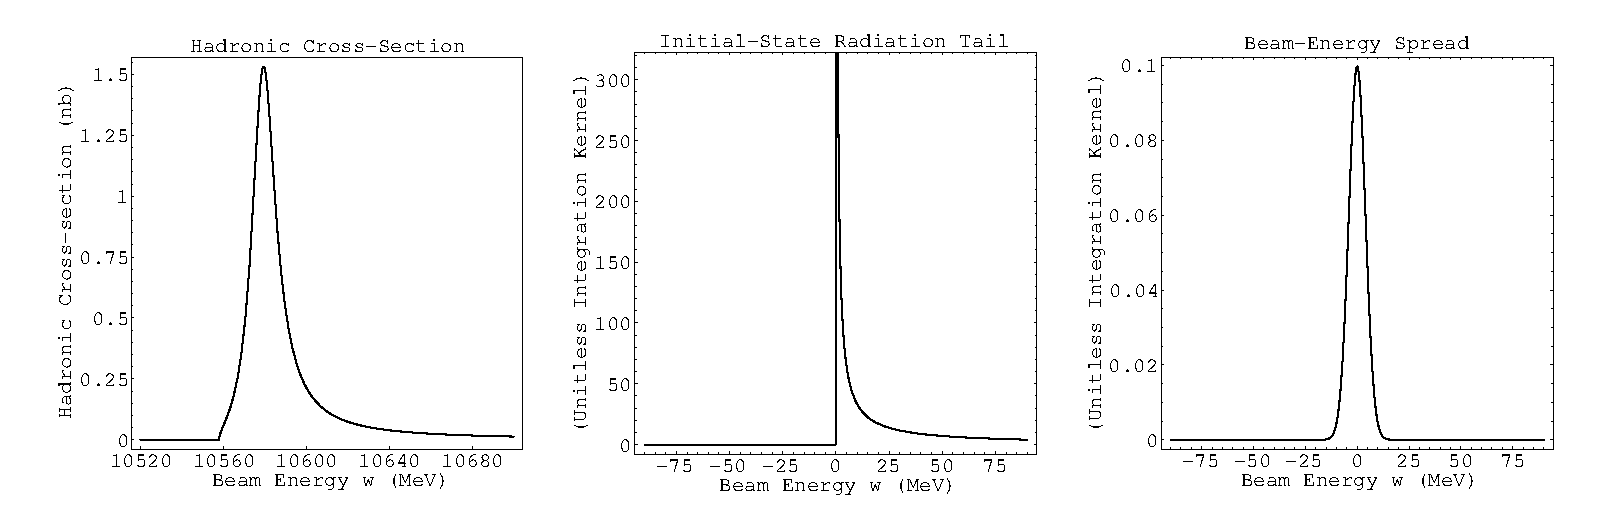
\includegraphics[width=\linewidth]{three_functions.eps}
  \end{center}

  \caption{The hadronic cross-section, initial-state radiation tail
  function and the beam energy spread, all to scale for the \yivs.
  (Each window is 180 MeV wide.)}

  \label{fig:3func}
\end{figure}

\noindent \label{page:other_backgrounds} All together, the observed
data is a three-way convolution of
\begin{enumerate}
  \item the hadronic cross-section line-shape
        $\sigma(w)_{\mbox{e$^+$e$^-$} \to \Upsilon\ \to \mbox{ hadrons}}$
  \item the initial-state radiation (ISR) tail (\ref{eq:kf}) and
  \item a unit Gaussian representing beam energy spread.
\end{enumerate}
These three functions are shown to scale (for the \yivs) in Figure
\ref{fig:3func}. The observed peak also sits on a $1/s$ pedistal of
continuum hadrons and tau-pair events, but this is easily removed.
Non-$1/s$ backgrounds like two-photon events, beam-gas, cosmic rays
and high-energy tails from the lower-lying resonances complicate
high-precision studies, but they can also be removed.

\subsection{What makes n = 4, 5, 6 so different?}

\begin{figure}[p]
  \begin{center}
    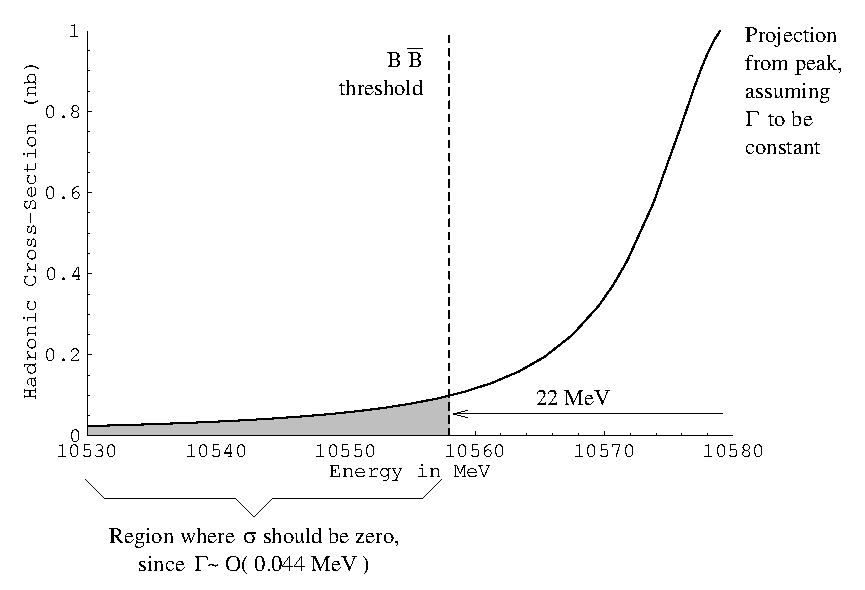
\includegraphics[width=0.75\linewidth]{bb_thresh.eps}
  \end{center}

  \caption{$\Gamma$ {\it must} vary significantly over the energies
  where the $\Upsilon(4S)$ hadronic cross-section is non-negligible,
  since it is 14 MeV at the peak and must be of order keV below the
  \bbar\ threshold.}

  \label{fig:bb_thresh}
\end{figure}

\begin{figure}[p]
  \begin{center}
    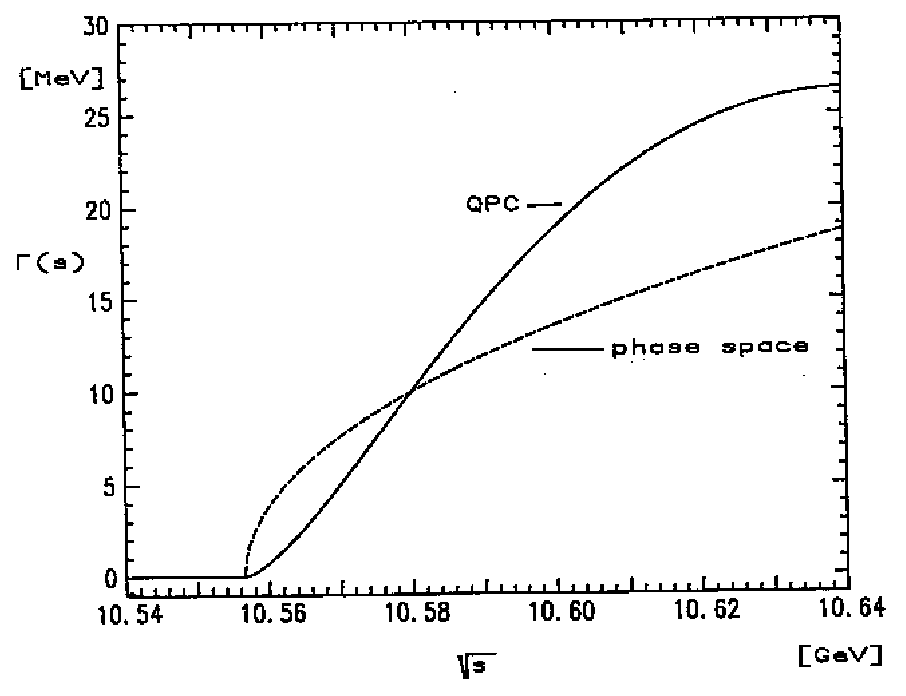
\includegraphics[width=0.45\linewidth]{gamma_from_models.eps}
    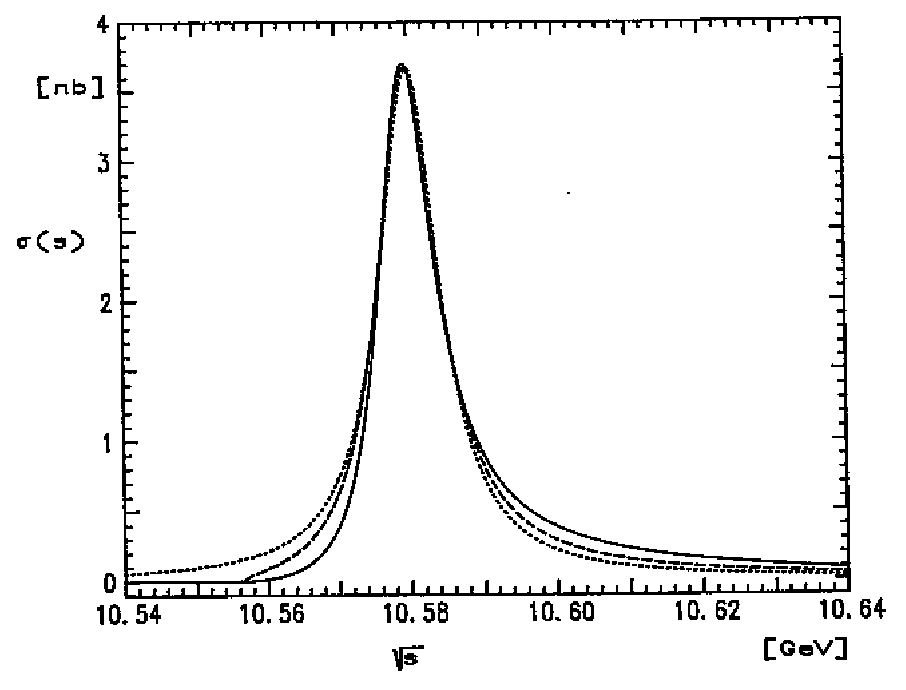
\includegraphics[width=0.45\linewidth]{peak_from_models.eps}
  \end{center}

  \caption{$\Gamma$ as a function of energy, and its effect on the
  line-shape of the \yivs. (From {\sc Argus} 1995 [\ref{cite:argus95}].) On
  the left, both functions have been normalized to have the same
  $\Gamma(\mbox{$M_\Upsilon$})$. On the right, the solid line uses
  the full QPC model, the dashed has only phase-space dependence and
  the dotted line is a Breit-Wigner ($\Gamma(s)$ is constant).}

  \label{fig:models}
\end{figure}

For the \yis, \yiis\ and \yiiis, we already know that the full width
\gamtot\ is narrow (order keV), so the hadronic cross-section
line-shape is a Breit-Wigner curve ([\ref{cite:ps}] p.\ 237). Having
identified all the contributions to the observed resonance peak, we
can parameterize a fit function and read off the line-shape area as
one of the fitted parameters.

The problem comes with $\Upsilon$ resonances above the mass of two $B$
mesons (n = 4 and up). Because these can easily decay into
\bbar-pairs, the hadronic width increases dramatically, and
\gamtot\ goes from tens of keV to tens of MeV. For these resonances,
the non-negligible hadronic cross-section spans over tens of MeV, and
\gamtot\ itself can vary over this energy scale. The shape of the peak
is now
\begin{equation}
  \sigma(w)_{\mbox{e$^+$e$^-$} \to \Upsilon\ \to \mbox{ hadrons}} =
  \frac{1}{\pi} \frac{\left(\Gamma(w)/2\right)
                     }{\left(w-\mbox{$M_\Upsilon$}\right)^2 + \left(\Gamma(w)/2\right)^2}
\end{equation}
where \gamofw\ is some as-yet unknown function of energy which
varies on the order of MeV.

As an illustration (Figure \ref{fig:bb_thresh}) of how necessary it is
to take this energy dependence into account, consider the \yivs, which
is close to the \bbar\ threshold. Near the peak, \gamofw\ is $\sim$14
MeV. If we extrapolate a curve from the peak with this width constant,
it crosses the \bbar\ threshold with a cross-section of about 0.1 nb
(not negligible). But below \bbar\ threshold, the resonance can't
decay into \bbar\ and its hadronic width must be order keV, so the
hadronic cross-section here should be about 0.0005 nb, a factor of 200
smaller! Somehow, this keV \gamofw\ must be matched up with an MeV
\gamofw, and this variation will distort the line-shape. Before a
fitting procedure can be prescribed, some \gamofw\ function will need
to be chosen.

The problem with choosing a \gamofw\ function is that the true
function depends quite a bit on the underlying dynamics. \gamofw\ is
proportional to the imaginary part of the $\Upsilon$ propogator
([\ref{cite:ps}] p.\ 237), which is governed by QCD. To calculate
\gamofw, one must either choose an effective model or do a lattice QCD
computation. In either case, the results of the experimental fit will
depend on some theory information as input, and this dependence will
need to be gauged.\label{page:old_method}

This procedure was used on the 1995 {\sc Argus} measurement of the
\yivs\ resonance [\ref{cite:argus95}]. The Quark Pair Creation (QPC)
model was chosen, and was compared to a simple phase-space model in
order to bound the bias. As can be seen in Figure \ref{fig:models},
\gamofw\ can differ by almost a factor of two.

This method is the best one I know, and more will be said of it later.
In the meantime, I have tried other methods to remove this dependence,
but all of them fail for one reason or another.

\subsection{Potential Measurement Strategies}

\subsubsection{Fitless Deconvolution (doesn't work)}

The simplest alternative is to avoid fitting altogether--- this way
there is no fit function to choose. Whatever the shape of
$\sigma(w)_{\mbox{e$^+$e$^-$} \to \Upsilon\ \to \mbox{ hadrons}}$, if
sample points are taken sufficiently close together, they can be
measured by a trapezoidal or Simpson's rule. The error introduced by
interpolation can easily be bounded, and one may even be able to find
an optimal scan strategy.

But the observed data is not a pure hadronic cross-section peak, it is
a convolution of this with beam energy spread and the ISR tail. The
beam energy spread convolution is not an issue: that has unit area and
areas multiply under convolutions. However, the ISR tail {\it is} a
problem--- it doesn't even have finite area.

We can apply the convolution theorem here:
\begin{eqnarray}
  \lefteqn{\mathcal{CONV}\left[ \sigma(w)_{\mbox{e$^+$e$^-$} \to \Upsilon\ \to \mbox{ hadrons}},\,
  \mbox{tail}(w) \right] =} \\
  \nonumber
  & & \mathcal{FT}^{-1} \left[
      \mathcal{FT}\left[ \sigma(w)_{\mbox{e$^+$e$^-$} \to \Upsilon\ \to \mbox{ hadrons}} \right] \times
      \mathcal{FT}\left[ \mbox{tail}(w) \right] \right]
\end{eqnarray}
where $\mathcal{FT}$ is a
Fourier Transform. We are only interested in the area (the origin in
Fourier-transformed space), so it becomes a matter of transforming two
functions, dividing their values at the origin and transforming back.

\begin{equation}
  \begin{array}{r c l}
    \mbox{area} &=& \displaystyle \int dw\,
      \mathcal{FT}^{-1} \left[
      \frac{\mathcal{FT}\left[ \mbox{observed data}(w) \right](z)}{\mathcal{FT}\left[ \mbox{tail}(w) \right](z)}
                       \right] \\
                & & \\
                &=& \displaystyle \int dw\, \int dz\,
      \frac{\mathcal{FT}\left[ \mbox{observed data}(w) \right](z)}{\mathcal{FT}\left[ \mbox{tail}(w) \right](z)}
      \, e^{2\pi i w z} \\
                & & \\
                &=& \displaystyle \int dz\, \left( \int dw\, e^{2\pi i w z} \right)
      \frac{\mathcal{FT}\left[ \mbox{observed data}(w) \right](z)}{\mathcal{FT}\left[ \mbox{tail}(w) \right](z)} \\
                & & \\
                &=& \displaystyle \int dz\, \bigg( \delta(z) \bigg) \,
      \frac{\mathcal{FT}\left[ \mbox{observed data}(w) \right](z)}{\mathcal{FT}\left[ \mbox{tail}(w) \right](z)} \\
                & & \\
                &=& \displaystyle \lim_{z \to 0}
      \frac{\int dw\, \mbox{observed data}(w) \, e^{-2\pi i w z}}{\int dw^{\prime}\, \mbox{tail}(w^{\prime}) \, e^{-2\pi i w^{\prime} z}}
  \end{array}
  \label{eq:alterarea_deriv}
\end{equation}
This limit can't be evaluated yet, since it would lead to an
indeterminant form. (The tail function, and therefore the observed
data, both have infinite area.)

We can consider cutting off both integrals at some high $W$. The ratio
then becomes
\begin{equation}
  \begin{array}{r c l}
    \mbox{area} &=& \displaystyle \lim_{z \to 0}
      \frac{\int_{-\infty}^W dw\, \mbox{observed data}(w) e^{-2\pi i w z} + X(W,z)}{
      \int_{-\infty}^W dw^{\prime}\, \mbox{tail}(w^{\prime}) e^{-2\pi i w^{\prime} z} + Y(W,z)} \\
      & & \\
                &\approx& \displaystyle \lim_{z \to 0}
      \frac{X(W,z)}{Y(W,z)}
  \end{array}
  \label{eq:alterarea}
\end{equation}
I still don't know how to evaluate this limit, but it is interesting
that the divergent nature of the radiative corrections allows me to
ignore the peak shape entirely. In fact, one could imagine an area
measurement where data is taken tens or hundreds of MeV above the
peak, and a few MeV below it (for background subtraction). The
``area'' is the observed cross-section at $w$ divided by
$\mbox{tail}(w)$, since the peak, whatever its shape, looks like a
delta function if $w - \mbox{$M_\Upsilon$} \gg \Gamma$. (This could
also be derived from (\ref{eq:alterarea}) by noting that the ratio of
areas is independent of the cut-off $W$, as long as $W$ is large.)

(I should make a technical note about units: peak area is expressed as
some cross-section (nb) times energy (MeV), and the above ratio is
only a cross-section (nb). The problem is that the delta function in
(\ref{eq:alterarea_deriv}) has units of energy, since it came from a
$dw$ integration. To do this calculation carefully, I would express
the tail function in its original form (\ref{eq:kf}), in terms of $f$,
the fractional photon energy, and I would express the data in the same
way. Then the delta function is unitless, and the desired area is a
number in nanobarns times the mass of the resonance, expressed in
whatever energy units you wish.)

\begin{figure}[h]
  \begin{center}
    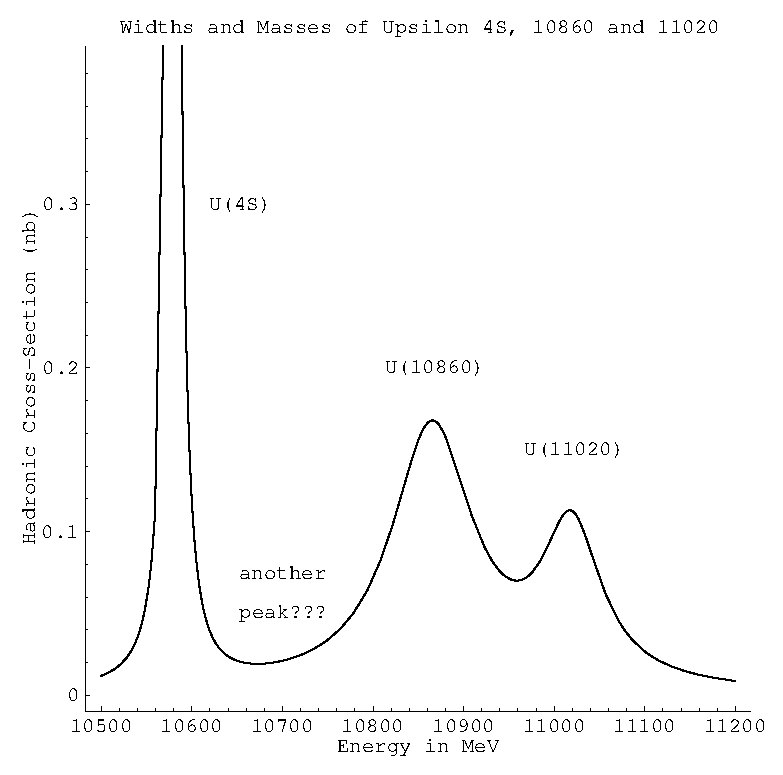
\includegraphics[width=0.35\linewidth]{theopeaks.eps}
    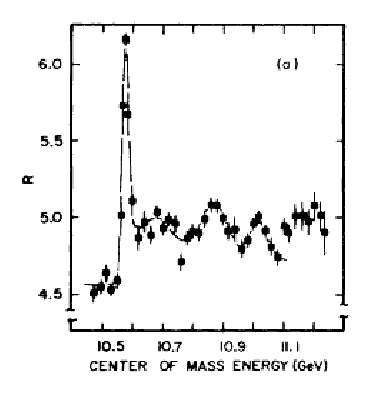
\includegraphics[width=0.35\linewidth]{exptpeaks.eps}
  \end{center}

  \caption{The three $\Upsilon$ states represented as Breit-Wigner
  curves with no $1/s$ pedistal, beam energy spread or QED
  corrections. This is to illustrate the relative widths and masses,
  and how much they overlap {\it before} all of that is included. On
  the right is the {\sc Cleo} 1985 data of the same region
  [\ref{cite:cleo85}], including the threshold effect on $R$ and the
  extra fitted bump at the \yivs.}

  \label{fig:theopeaks}
\end{figure}

Something like this might have worked for the \yis, \yiis\ or \yiiis.
It would have traded concerns about beam energy calibration for poor
statistics at the sample point, especially when continuum-subtracted
and divided by the less-than-unity tail function (not to mention other
backgrounds mentioned on page \pageref{page:other_backgrounds}--- at
least one scan of each lower resonance would be needed to remove their
ISR contributions).

But such a method can't be used for the n = 4, 5, 6 resonances, since
there are no wide, empty gaps between them. Figure \ref{fig:theopeaks}
shows the n = 4, 5, 6 environment as an overlapping set of
Breit-Wigner resonances. Because this ignores smearing due to beam
energy and \gamofw\ dependence, this actually {\it underestimates} the
overlap between resonances.

A fitting procedure will be needed to extract the peak areas
(especially \yvs\ and \yvis), so I will need to know something about
\gamofw.

\subsubsection{Directly measure \gamofw\ (doesn't work)}

If I have to fit, perhaps I can find \gamofw\ some way that doesn't
resort to a theoretical prediction. A possibility I considered was to
do a \bree\ (or \brmumu) measurement at every sample point. While
\gamofw\ is known to vary on the scale of MeV, \gamee\ should be
$1/\sqrt{s}$. Therefore, if we knew \bree, we would know \gamofw\ 
through
\begin{equation}
  \Gamma(w) = \frac{\Gamma_{ee}}{\mathcal{BR}_{ee}(w)}
\end{equation}

The problem is that \bree\ is very hard to measure (independently of
\gamee) for the wide resonances: $\mathcal{BR}_{ee} =
N_{ee}/N_{\mbox{tot}} = 2\times10^{-5}$. For a reasonable
($\mathcal{O}(1\%)$) uncertainty,
\begin{equation}
  \frac{\sigma_{\mathcal{BR}_{ee}}}{\mathcal{BR}_{ee}} =
  \sqrt{\frac{1}{N_{ee}} + \frac{1}{N_{\mbox{tot}}}} =
  \sqrt{\frac{1}{N_{\mbox{tot}}}} \sqrt{\frac{1}{\mathcal{BR}_{ee}} + 1}
\end{equation}
\begin{center} or \end{center}
\begin{equation}
  N_{\mbox{tot}} =
  \frac{1/\mathcal{BR}_{ee}}{\left(\frac{\sigma_{\mathcal{BR}_{ee}}}{\mathcal{BR}_{ee}}\right)^2} =
  \frac{\frac{1}{2}\times 10^5}{\left(0.01\right)^2} =
  5\times 10^8 \mbox{ } \Upsilon \mbox{ events}
\end{equation}
which is unattainable, particularly at enough scan points to map out a
curve.

\subsubsection{Let $d\Gamma/dw\big|_{w=\mbox{$M_\Upsilon$}}$ float (doesn't work)}
\label{sec:float_slope}

The last alternate method I considered was to replace the full
function \gamofw\ with an expansion around its value at the peak. So
\begin{equation}
  \Gamma(w) = \Gamma_0 + \Gamma_1 (w - \mbox{$M_\Upsilon$})
\end{equation}
where $\Gamma_0$ and $\Gamma_1$ are two free parameters in the fit.

But the need to know about \gamofw\ far from the peak still creeps in,
in two different ways. The subtle way is the fact that ISR will spread
some of the cross-section from the left-hand side of the peak up to
higher energies--- some of the cross-section at $M_\Upsilon$ will come
from the threshold region, where \gamofw\ is unknown. The
show-stopping way is the fact that without knowing the whole \gamofw\ 
curve, I can't reconstruct the area of the whole peak from a fit to a
part of the peak.

\subsubsection{Assume \gamofw\ from theory (what was done before)}

Out of options, I return to the method that was used before. (This was
described first on page \pageref{page:old_method}.) The shape of
\gamofw\ is calculated theoretically, and is then parameterized by an
overall scale $\Gamma(w=\mbox{$M_\Upsilon$})$, which is allowed to
float in the fit. The scale of the bias is bounded by fitting again
with the \gamofw\ dependence removed, or replaced by a very different
model.

The {\sc Argus} measurement at the \yivs\ [\ref{cite:argus95}]
involved such a procedure, where the Quark Pair Creation model was
compared to a ``nothing but phase-space'' model. (This is a rather
large difference in \gamofw! see Figure \ref{fig:models}.) The results
for \gamee\ differed by about 5\%, making 5\% an upper bound on the
theory-bias systematic at the \yivs. One would need to know more about
the validity of the model in question to get a better estimate on the
true error, which is probably much smaller than this.
\label{page:fit_systematic}

(It should be noted that if lattice QCD is used to calculate \gamofw,
this compromises the final measurement of \gamee\ as a precision test
for lattice QCD. One could imagine a scenario in which lattice QCD is
used to calculate \gamofw, and a $\sim$10\% uncertainty in the lattice
calculation is used to claim a 1\% systematic in \gamee. (My
estimation comes from the $\sim$50\% difference between QPC and
phase-space yielding a 5\% systematic in \gamee.) A 1\% lattice
calculation of \gamee\ at the \yivs\ can't be compared to the \gamee\ 
measurement at a 1\% level, but at 5\%, the appropriate level of
precision with no theory input.)

\subsubsection{Freedom from theory at the \yvs\ and \yvis}

These concerns may be almost negligible at the very high resonances,
\yvs\ and \yvis, since they are far above the \bbar\ threshold and
\gamofw\ asymtotically approaches the phase-space model. In fact, even
the variation of \gamofw\ with $w$ ($d\Gamma/dw$) is 20\% of what it
is at the \yivs.

\label{page:freedom}
Considering this, it is possible to salvage the method described in
subsection \ref{sec:float_slope}. Parameterize \gamofw\ as a deviation
from phase-space:
\begin{equation}
  \Gamma(w) = \Gamma_0 \, \frac{\sqrt{w^2 - (2 M_B)^2}}{w^2} + \Gamma_1 \, (w - \mbox{$M_\Upsilon$})
\end{equation}
The size of the fitted correction term compared to the phase-space
term (at about one or two half-widths from the peak) should tell you
if a quadratic term is needed.

% \begin{equation}
%   \frac{d \Gamma_{\mbox{phase space}}}{dw}\big|_{w=\mbox{$M_\Upsilon$}} =
%   \frac{8 \mbox{$M_B$}^2 - \mbox{$M_\Upsilon$}^2}{\mbox{$M_\Upsilon$}^3
%     \sqrt{\mbox{$M_\Upsilon$}^2 - 4 \mbox{$M_B$}^2}}
% \end{equation}

Due to the overlap, the \yvs\ and \yvis\ will need to be fitted
together. The fit will include ten parameters in all: area,
$\Gamma_0$, $\Gamma_1$, mass, beam energy spread and pedistal for the
\yvs, area, $\Gamma_0$, $\Gamma_1$, and mass for the \yvis. Beam
energy spread may even be neglected, as it should be about 5 MeV where
\gamtot\ is about 100 MeV.

\subsection{Measurements to Date}

The 1995 {\sc Argus} measurement has already been discussed, but that
scan only includes the \yivs. For the \yvs\ and \yvis, one needs to go
back to the scans obtained concurrently by {\sc Cleo} and {\sc Cusb}
in 1985. A summary of these results is presented below. {\sc Cusb}
didn't publish systematic and statistical uncertainties seperately, so
I don't know if the 13\% measurement claimed at the \yivs\ can be
considered more precise than the 18\% measurement by {\sc Argus}, ten
years later.

\begin{center}
  \begin{tabular}{c | l | c | c}
    Resonance & Detector & $\Gamma_{ee}$ & Uncertainty \\\hline\hline
    4S & {\sc Cleo} 1985 [\ref{cite:cleo85}] & $0.192 \pm 0.007 \pm 0.038$ & 20\% \\
       & {\sc Cusb} 1985 [\ref{cite:cusb85}] & $0.283 \pm 0.037$ & 13\% \\
       & {\sc Argus} 1995 [\ref{cite:argus95}] & $0.28 \pm 0.05 \pm 0.01$ & 18\% \\\hline

    10860 & {\sc Cleo} 1985 & $0.22 \pm 0.05 \pm 0.07$ & 40\% \\
          & {\sc Cusb} 1985 & $0.365 \pm 0.070$ & 19\% \\\hline

    11020 & {\sc Cleo} 1985 & $0.095 \pm 0.03 \pm 0.035$ & 48\% \\
          & {\sc Cusb} 1985 & $0.156 \pm 0.040$ & 26\% \\
  \end{tabular}
\end{center}

\subsection{Limiting Systematics}

The systematic error due to choice of fit function has been discussed,
it has already been bounded at 5\%. But this 5\% is larger than it
needs to be, supposing that the uncertainty in the theoretical
prediction of \gamofw\ can be more rigorously bounded, or a method
such as the one described on page \pageref{page:freedom} is used for
the \yvs\ and \yvis. Then the next largest systematic uncertainty is
the uncertainty in {\sc Cleo III} luminosity measurement, currently
quoted as 2\%, but reducible to 1\% at least, since $\Upsilon \to
\mbox{e$^+$e$^-$}$ is insignificant at the \yivs, \yvs\ and \yvis.
(This effect accounts for a 1.1\% bias at the \yis, \yiis\ and
\yiiis.)

% Therefore, I will consider statistical uncertainties down to 1\% as
% reasonable goals, but no less.

\subsection{How much {\sc Cleo III} Luminosity is Needed for a Better Measurement?}

\begin{figure}[t]
  \begin{center}
    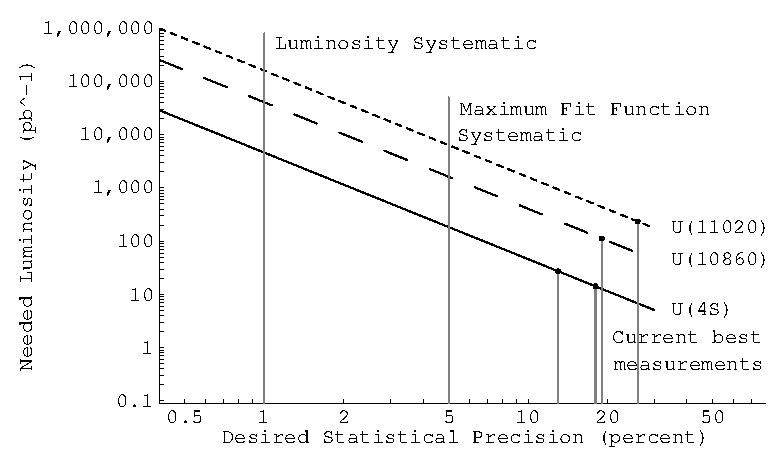
\includegraphics[width=0.75\linewidth]{cleo_lumi_needed.eps}
  \end{center}

  \caption{Integrated luminosity needed to obtain a given statistical
  precision. The solid line represents the luminosity needed to fit a
  \yivs\ resonance to the desired precision. The dashed and dotted
  lines each represent the luminosity needed for a combined
  \yvs--\yvis\ scan.}

  \label{fig:lumi}
\end{figure}

If we would like to improve upon this measurement at {\sc Cleo III}, I
will need to provide some conversion between {\sc Cleo} integrated
luminosity and uncertainty in \gamee.

Since \gamee\ is directly proportional to $\int dw\,
\sigma_{\mbox{e$^+$e$^-$} \to \Upsilon\ \to \mbox{ hadrons}}$, a
fractional uncertainty in one is the fractional uncertainty in the
other. Estimating the luminosity needed to achieve a given area
uncertainty is complicated by the fact that the resonances are not
boxes. Therefore, I did a series of fits to correctly-parameterized
Breit-Wigner distributions (with pedistal), evenly divided into
forty-five bins. Because the \yvs\ and \yvis\ overlap significantly, I
fitted these two resonances together, also in forty-five bins.

For the \yivs, I obtained the following empirical relationship between
desired precision and luminosity:
\begin{equation}
  \mbox{desired precision} = \mbox{3.2\%} \sqrt{\frac{\mbox{450 pb$^{\mbox{\small -1}}$}}{\mathcal{L}}}
  \hspace{3mm} \mbox{ or } \hspace{3mm} 
  \mathcal{L} = \mbox{450 pb$^{\mbox{\small -1}}$} \left(\frac{\mbox{3.2\%}}{\mbox{desired precision}}\right)^2
\end{equation}
This is reasonable, since uncertainty in hadronic cross-section at one
sample point scales with luminosity as $1/\sqrt{\mathcal{L}}$. This
relationship is represented by the solid line in Figure
\ref{fig:lumi}. A scan program that puts 200 pb$^{\mbox{\small -1}}$ on the
\yivs\ peak would reach a statistical precision of 5\%, and this could
be the dominating systematic if the theoretical form of the fit
function is better bounded. A 2\%-level measurement would require
about 5000 pb$^{\mbox{\small -1}}$.

A \yvs\ and \yvis\ scan yields this relationship:
\begin{equation}
  \begin{array}{r c l}
  \displaystyle \mathcal{L}_{\mbox{scan over both peaks}} &=& \displaystyle \mbox{45,000 pb$^{\mbox{\small -1}}$}
    \left(\frac{\mbox{0.95\%}}{\mbox{desired \yvs\ precision}}\right)^2 \\
  & & \\
  &=& \displaystyle \mbox{45,000 pb$^{\mbox{\small -1}}$}
    \left(\frac{\mbox{1.88\%}}{\mbox{desired \yvis\ precision}}\right)^2
  \end{array}
\end{equation}
The 1:2 relationship between the precision at the \yvs\ and the
precision at the \yvis\ is a consequence of the evenly-spaced and
evenly-sampled data points. One could devise a scan plan that puts
more data on the higher resonance to balance the statistical
uncertanties. In Figure \ref{fig:lumi}, the dashed line shows how much
luminosity must be put into the combined \yvs--\yvis\ scan to achieve
a given statistical precision in \gamee\ for the \yvs. The dotted line
shows the combined luminosity for a given precision in \gamee\ for the
\yvis.

Here it will be hard to do better than the current best measurements,
since this would require orders of magnitude more data than the \yis,
\yiis, \yiiis\ scan program. For a 5\%:10\% measurement, one would need
about 2,000 pb$^{\mbox{\small -1}}$. For a 1\%:2\% measurement, one would
need about 30,000 pb$^{\mbox{\small -1}}$.

The 1985 {\sc Cleo} measurement makes a good check of this predicted
relationship between statistical precision and luminosity, because
statistical uncertainties and integrated luminosities were both quoted
[\ref{cite:cleo85}]. This paper also divides the scans into ``\yivs''
and ``\yvs--\yvis.''
\begin{center}
  \begin{tabular}{c | c c c}
    & Luminosity & Predicted Statistical Precision & Actual Precision \\\hline
    \yivs & 40.6 pb$^{\mbox{\small -1}}$ & 11\% & 36\% \\
    \yvs & part of 70 pb$^{\mbox{\small -1}}$ & 24\% & 22\% \\
    \yvis & part of 70 pb$^{\mbox{\small -1}}$ & 48\% & 32\% \\
  \end{tabular}
\end{center}
There is only a rough agreement--- a factor of 2 to 4. Whatever the
constant, I believe the $1/\sqrt{\mathcal{L}}$ dependence, so I will project
this discrepancy to higher luminosities with the following:
\begin{equation}
  L = \frac{\mbox{const}}{\%^2} \hspace{1cm}
  \partial L = -2\,\frac{\mbox{const}}{\%^3}\,\partial \% \hspace{1cm}
  \mbox{so } \frac{\partial L}{L} = -2\,\frac{\partial \%}{\%}
\end{equation}
These predictions should only be trusted to a factor of two to four at
any luminosity.

\subsection{References}

\begin{enumerate}

  \item Peskin and Schroeder {\it An Introduction to Quantum Field
  Theory}, Perseus Books Publishing, L.~L.~C. 1995. \label{cite:ps}

  \item E.~A.~Kuraev and V.~S.~Fadin,
  	``On Radiative Corrections To E+ E- Single Photon Annihilation At High-Energy,''
  	Sov.\ J.\ Nucl.\ Phys.\  {\bf 41}, 466 (1985)
  	[Yad.\ Fiz.\  {\bf 41}, 733 (1985)]. \label{cite:kf}

  \item H.~Albrecht {\it et al.}  [ARGUS Collaboration],
	``A Measurement of the electronic widths gamma (e e) of the upsilon (1s), upsilon (2s),
          and upsilon (4s) resonances, and of the total decay
	width Gamma of the upsilon (4s),''
	Z.\ Phys.\ C {\bf 65}, 619 (1995). \label{cite:argus95}

  \item D.~M.~Lovelock {\it et al.},
	``Masses, Widths, And Leptonic Widths Of The Higher Upsilon Resonances,''
	Phys.\ Rev.\ Lett.\  {\bf 54}, 377 (1985). \label{cite:cleo85}

  \item D.~Besson {\it et al.}  [CLEO Collaboration],
	``Observation Of New Structure In The E+ E- Annihilation Cross-Section Above B Anti-B Threshold,''
	Phys.\ Rev.\ Lett.\  {\bf 54}, 381 (1985). \label{cite:cusb85}

\end{enumerate}

\end{document}





% Breit-Wigner curves have $\mbox{area} = \pi/2\, \mbox{peak} \,
% \Gamma$, so if \gamtot is well-known, the fractional uncertainty in
% area will be roughly the fractional uncertainty in the peak value,
% assuming all data to be taken at the peak. Uncertainties in area and
% \gamtot\ will be correlated, of course, but I am only trying to get an
% order-of-magnitude estimate for the necessary luminosity.

% Hadronic cross-section (hxs) is related to luminosity by $\mbox{hxs} =
% N_{\mbox{hadrons}} / \mathcal{L}$, and luminosity is related to the
% number of bhabhas collected as $\mathcal{L} = L_0 \,
% N_{\mbox{bhabhas}}$, where $L_0 = $ 0.0759
% nb$^{\mbox{-1}}/\mbox{event}$ for {\sb Cleo III}. Luminosity
% uncertainty is therefore
% \begin{equation}
%   \sigma_{\mathcal{L}} = L_0 \, \sqrt{N_{\mbox{bhabhas}}} = \sqrt{L_0 \, \mathcal{L}}
%   \mbox{ or }
%   \frac{\sigma_{\mathcal{L}}}{\mathcal{L}} = \sqrt{\frac{L_0}{\mathcal{L}}}
% \end{equation}
% and hadronic cross-section uncertainty is
% \begin{equation}
%   \frac{\sigma_{\mbox{hxs}}}{\mbox{hxs}} = \sqrt{\frac{1}{N_{\mbox{hadrons}}} +
%     \left(\frac{\sigma_{\mathcal{L}}}{\mathcal{L}}\right)^2}
%   = \sqrt{\frac{1}{\mbox{hxs} \, \mathcal{L}} + \frac{L_0}{\mathcal{L}}}
%   = \sqrt{\frac{1}{\mathcal{L}}} \, \sqrt{\frac{1}{\mbox{hxs}} + L_0}
% \end{equation}

% This hadronic cross-section is assumed to be that at the peak after
% background subtraction. To do the background subtraction, twice the
% luminosity will be needed, so
% \begin{equation}
%   \mathcal{L} = \frac{\left(\frac{1}{\mbox{hxs}}\right)}{2
%     \, \left(\frac{\sigma_{\mbox{hxs}}}{\mbox{hxs}}\right)^2}
% \end{equation}

% Figure \ref{fig:lumi} shows the needed luminosity as a function of
% desired statistical precision. It would be fairly easy to improve upon
% the \yivs\ scan, a 1\% statistical measurement would only cost 20
% pb$^{\mbox{\small -1}}$. The \yvs\ and \yvis\ are harder to measure because
% they don't stand as high above the background, due to their extreme
% widths. Nevertheless, they can be measured to a 1\% statistical
% precision with 200--300 pb$^{\mbox{\small -1}}$, 2\% with 50 pb$^{\mbox{\small -1}}$
% or a 5\% statistical precision with 7--8 pb$^{\mbox{\small -1}}$. The 1\%
% statistical precision measurements 
